\section{Supplementary material}
\label{sec:supplementary_material}

\begin{figure}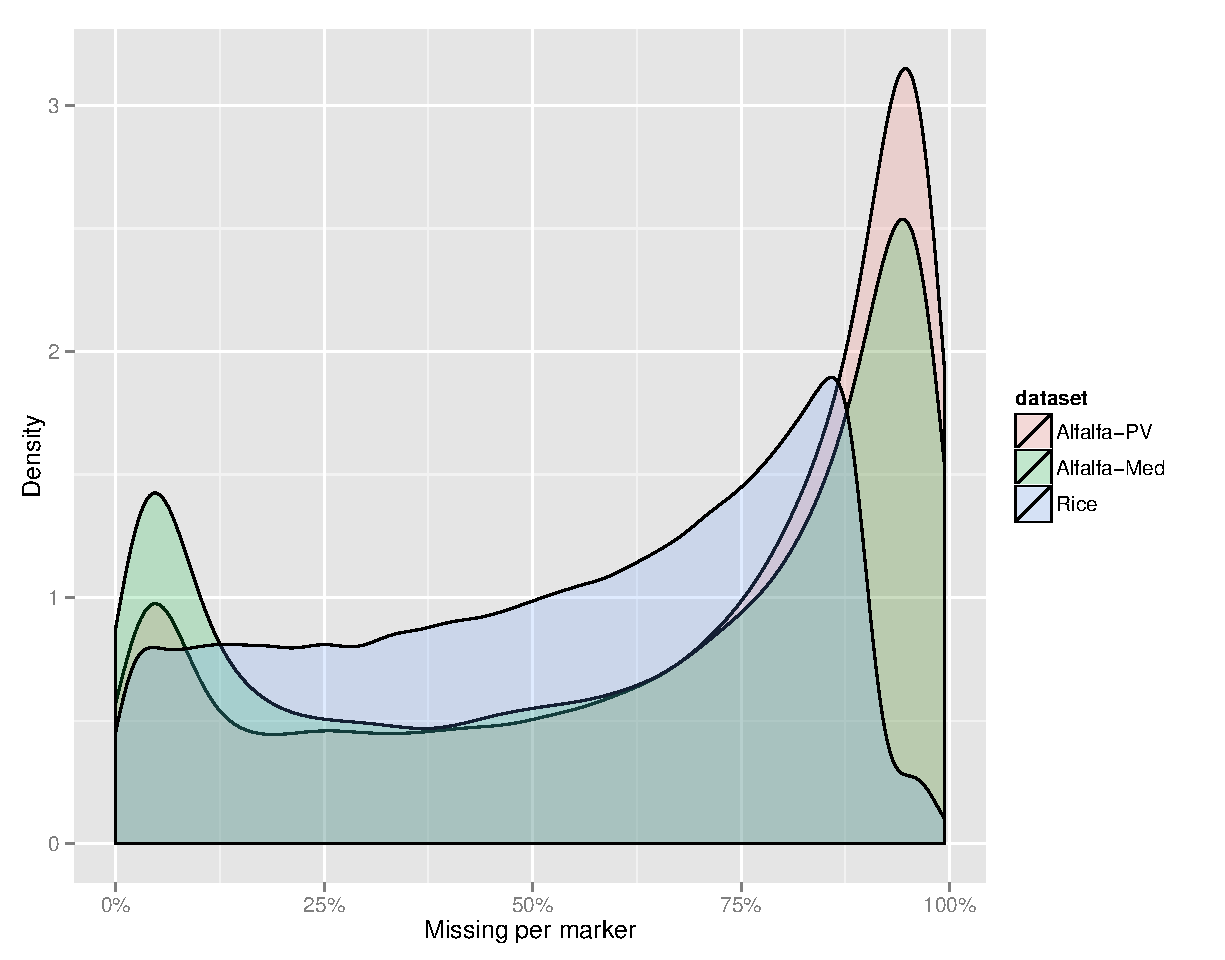
\includegraphics[width=0.95\textwidth]{SupplFig01_miss_per_marker.pdf}
\caption{Distribution of missings-per-marker rates in the three datasets. This is a
density plot, so all curves delimit the same unitary area.}
\end{figure}

\begin{figure}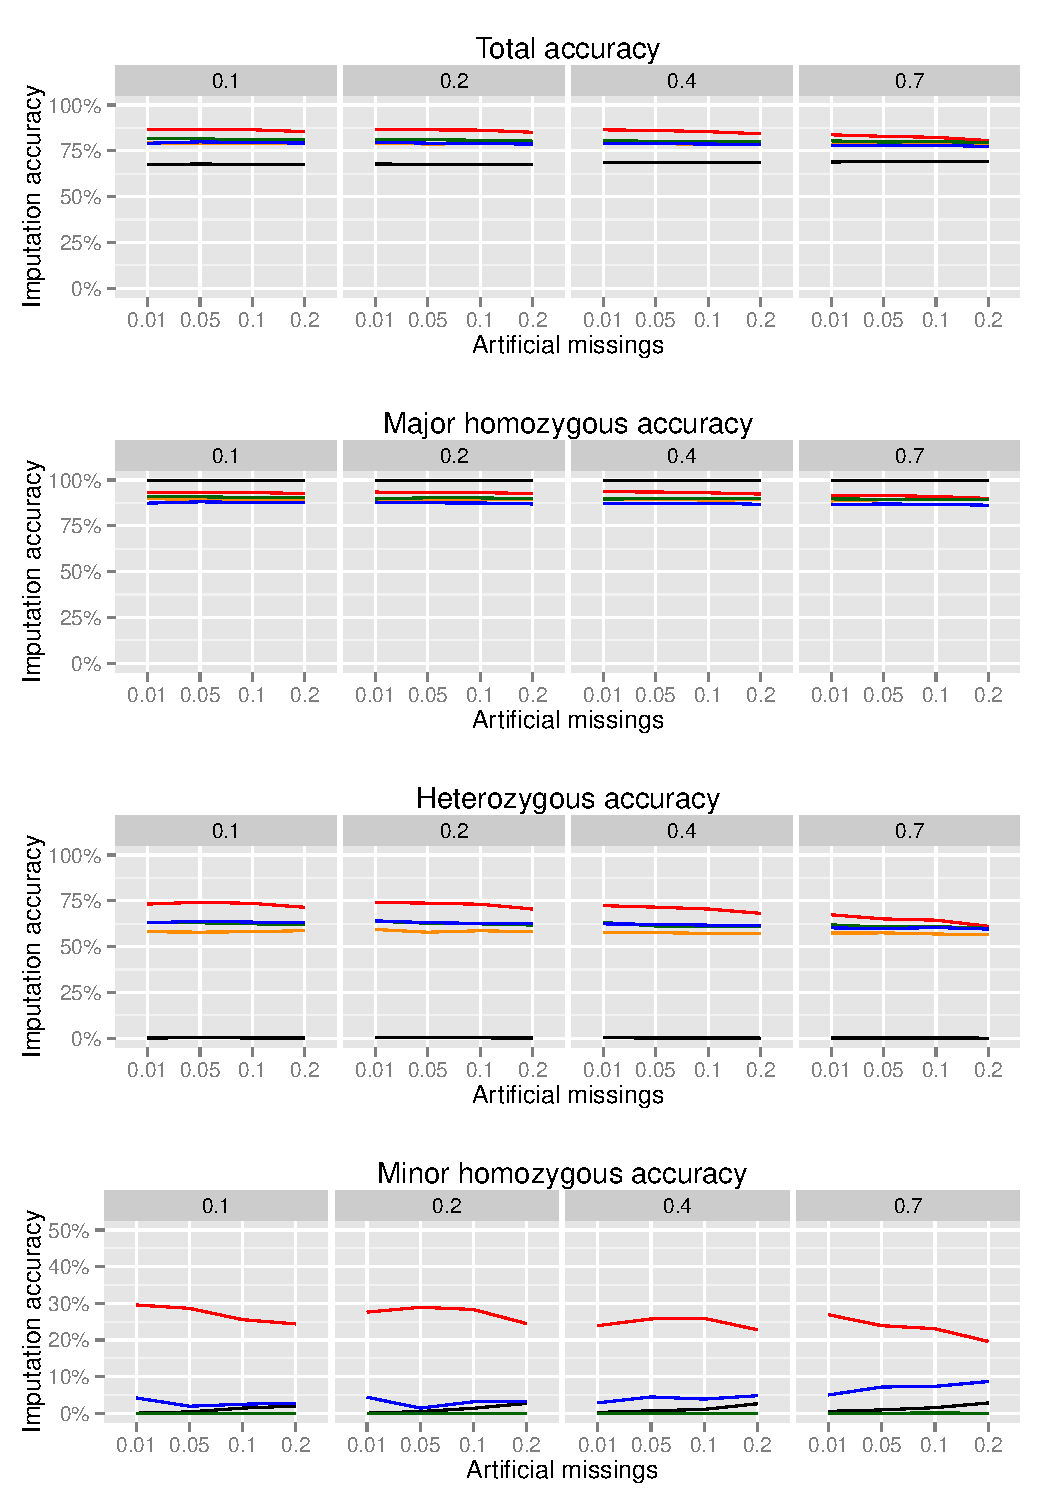
\includegraphics[width=0.95\textwidth]{SupplFig02_Alfalfa-Med.pdf}\caption{
imputation accuracies overall, for the major homozygous genotype (AA), for heterozygotes (AB), and for the minor homozygous genotype (BB) in datasets consisting of
10\%, 20\%, 40\% and 70\% allowed missing data per locus (boxes) with 1\%, 5\%, 10\% and 20\%
additional missing values artificially introduced (x-axis) for alfalfa population Alfalfa-Med.
Lines colors represent the five imputation algorithms: MNI
(orange), KNNI (red), SVDI (blue), RFI (green) and Beagle (black)}\end{figure}
\begin{figure}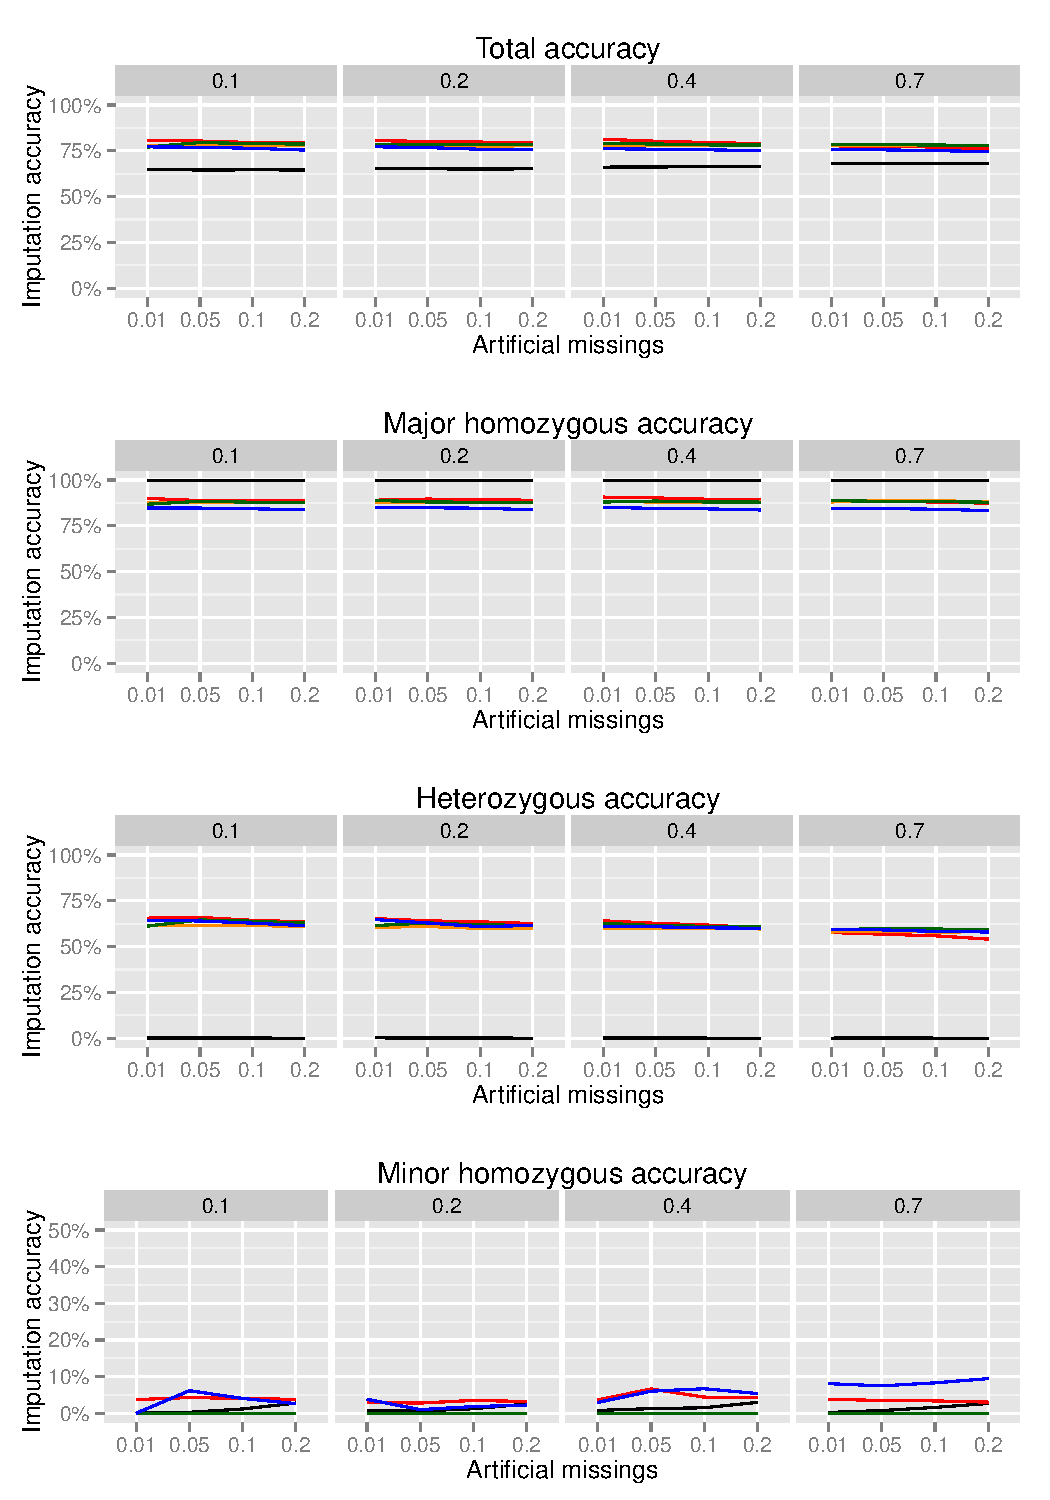
\includegraphics[width=0.95\textwidth]{SupplFig03_Alfalfa-PV.pdf}\caption{
imputation accuracies overall, for the major homozygous genotype (AA), for heterozygotes (AB), and for the minor homozygous genotype (BB) in datasets consisting of
10\%, 20\%, 40\% and 70\% allowed missing data per locus (boxes) with 1\%, 5\%, 10\% and 20\%
additional missing values artificially introduced (x-axis) for alfalfa population Alfalfa-PV.
Lines colors represent the five imputation algorithms: MNI
(orange), KNNI (red), SVDI (blue), RFI (green) and Beagle (black)}\end{figure}
\begin{figure}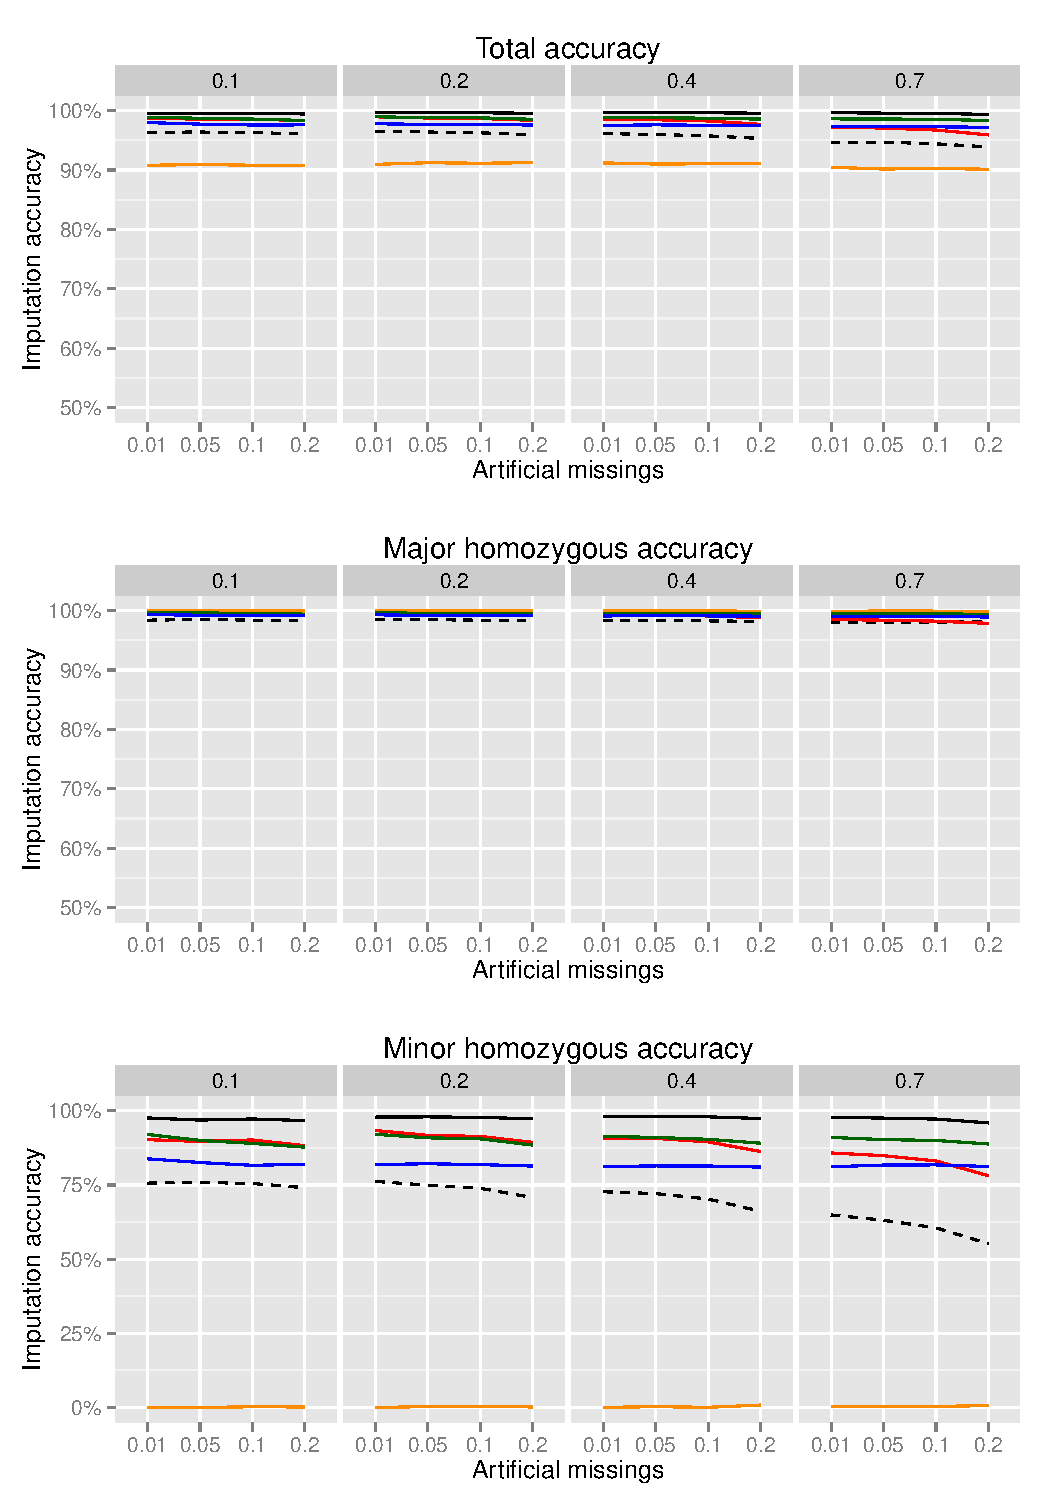
\includegraphics[width=0.95\textwidth]{SupplFig04_Rice-chrom-1.pdf}\caption{
imputation accuracies overall, for the major homozygous genotype (AA) and for the minor homozygous genotype (BB) in datasets consisting of
10\%, 20\%, 40\% and 70\% allowed missing data per locus (boxes) with 1\%, 5\%, 10\% and 20\%
additional missing values artificially introduced (x-axis) for rice chromosome 1 data.
Lines colors represent the five imputation algorithms: MNI
(orange), KNNI (red), SVDI (blue), RFI (green) and Beagle (black)}\end{figure}
\begin{figure}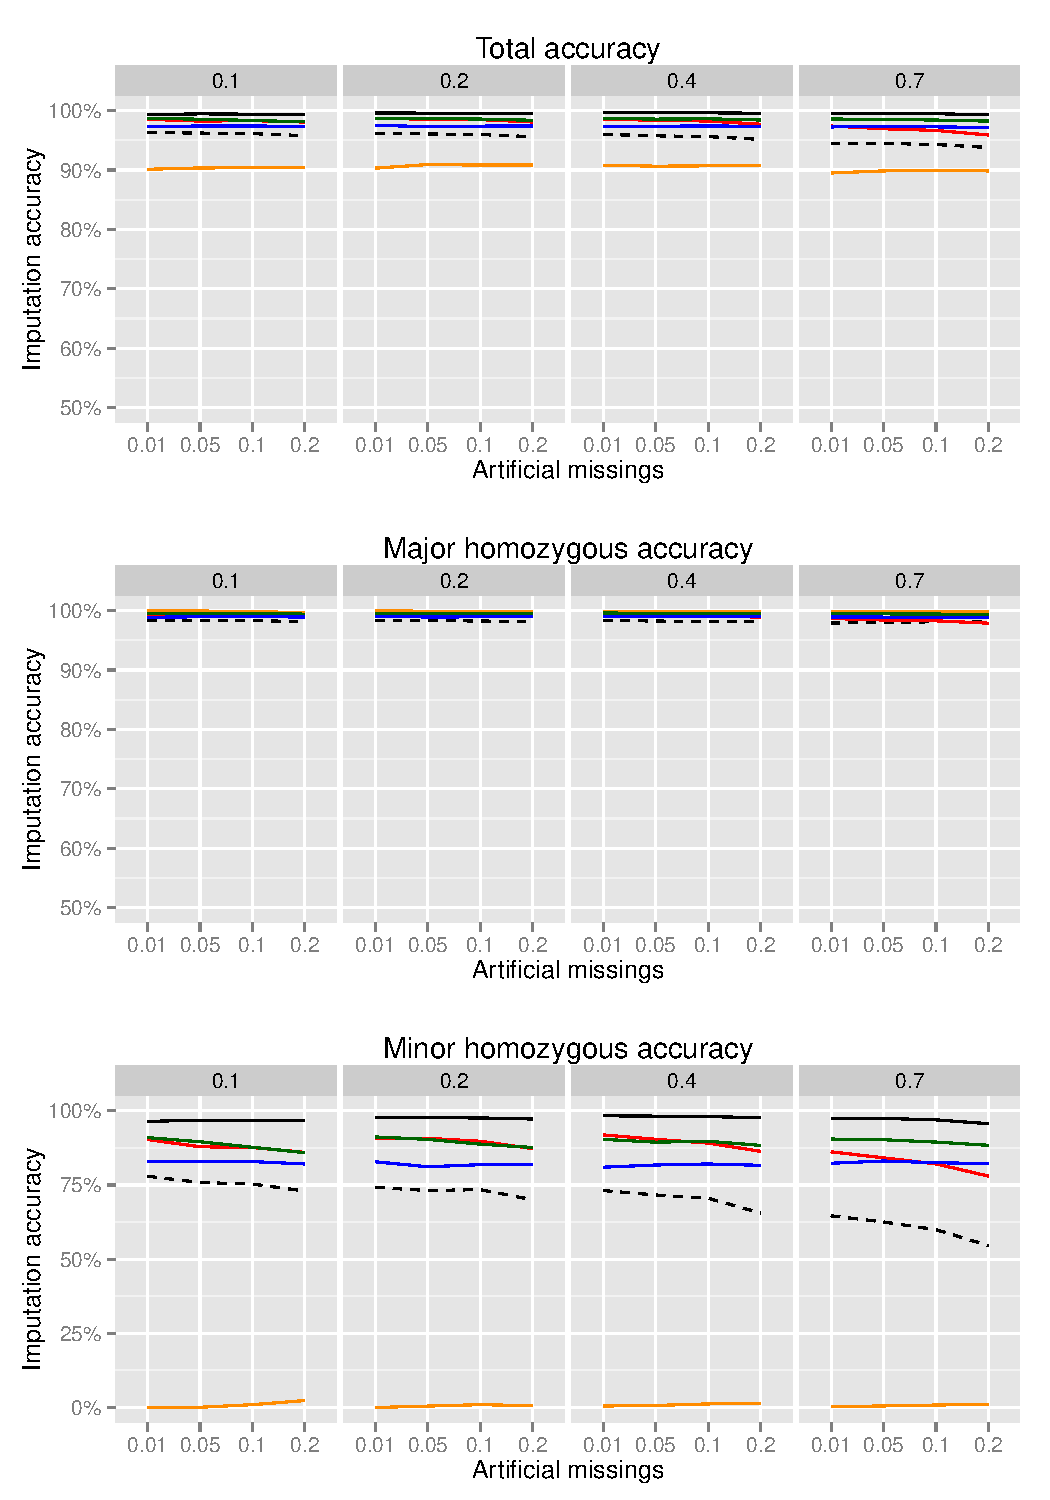
\includegraphics[width=0.95\textwidth]{SupplFig05_Rice-chrom-2.pdf}\caption{
imputation accuracies overall, for the major homozygous genotype (AA) and for the minor homozygous genotype (BB) in datasets consisting of
10\%, 20\%, 40\% and 70\% allowed missing data per locus (boxes) with 1\%, 5\%, 10\% and 20\%
additional missing values artificially introduced (x-axis) for rice chromosome 2 data.
Lines colors represent the five imputation algorithms: MNI
(orange), KNNI (red), SVDI (blue), RFI (green) and Beagle (black)}\end{figure}
\begin{figure}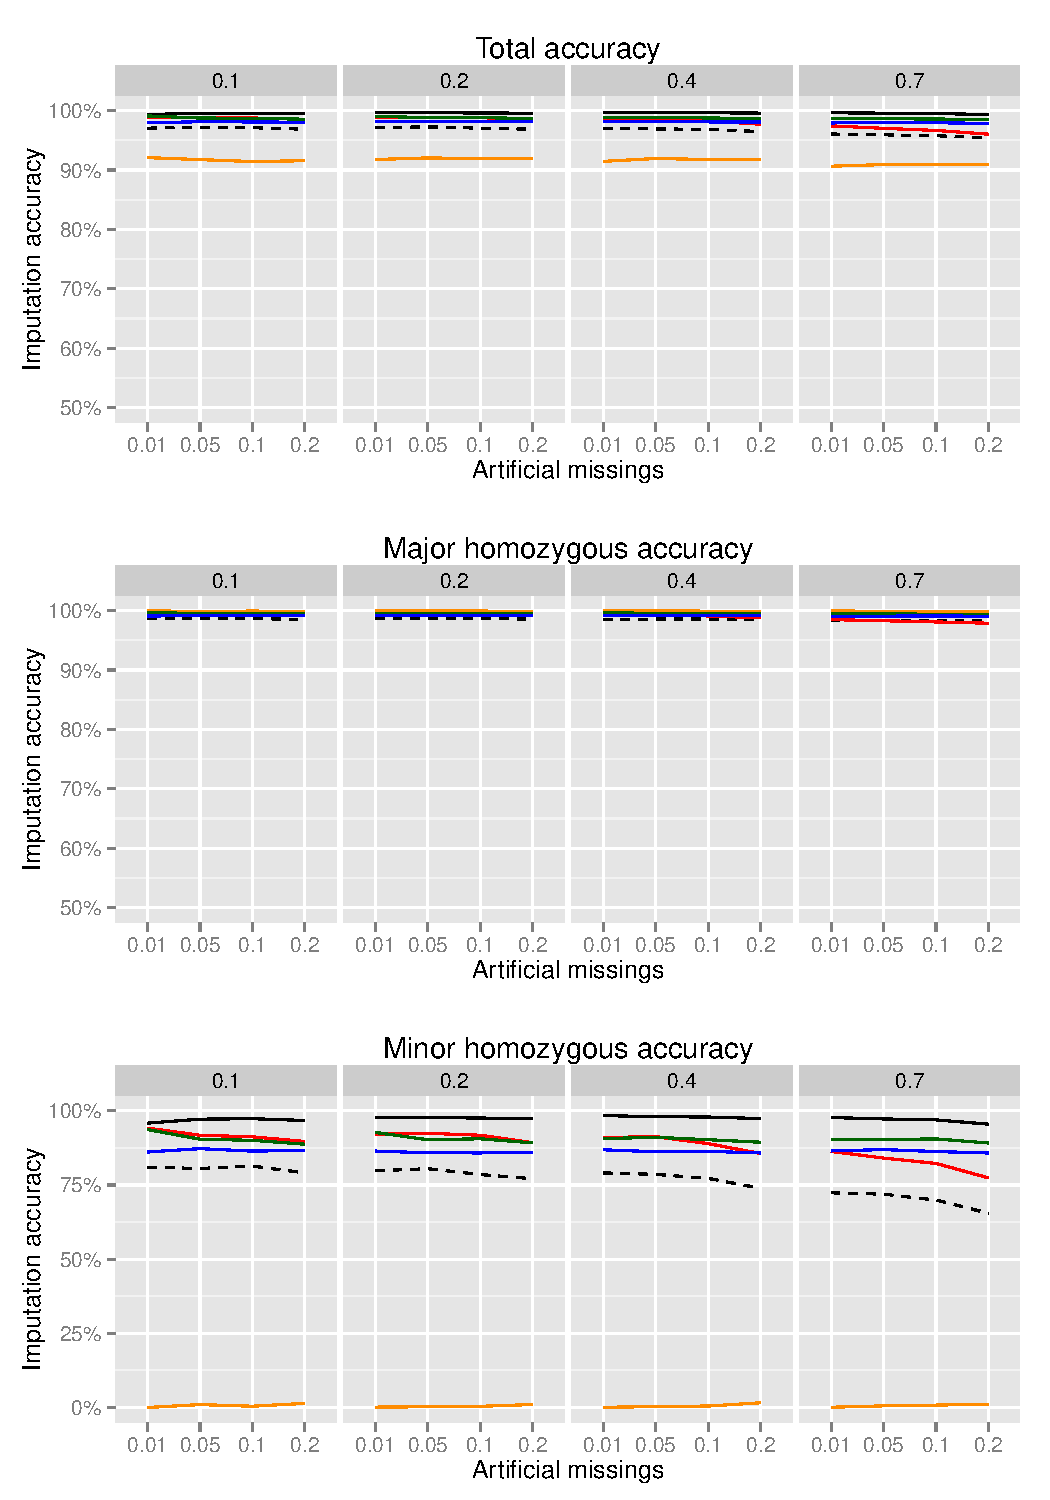
\includegraphics[width=0.95\textwidth]{SupplFig06_Rice-chrom-3.pdf}\caption{
imputation accuracies overall, for the major homozygous genotype (AA) and for the minor homozygous genotype (BB) in datasets consisting of
10\%, 20\%, 40\% and 70\% allowed missing data per locus (boxes) with 1\%, 5\%, 10\% and 20\%
additional missing values artificially introduced (x-axis) for rice chromosome 3 data.
Lines colors represent the five imputation algorithms: MNI
(orange), KNNI (red), SVDI (blue), RFI (green) and Beagle (black)}\end{figure}
\begin{figure}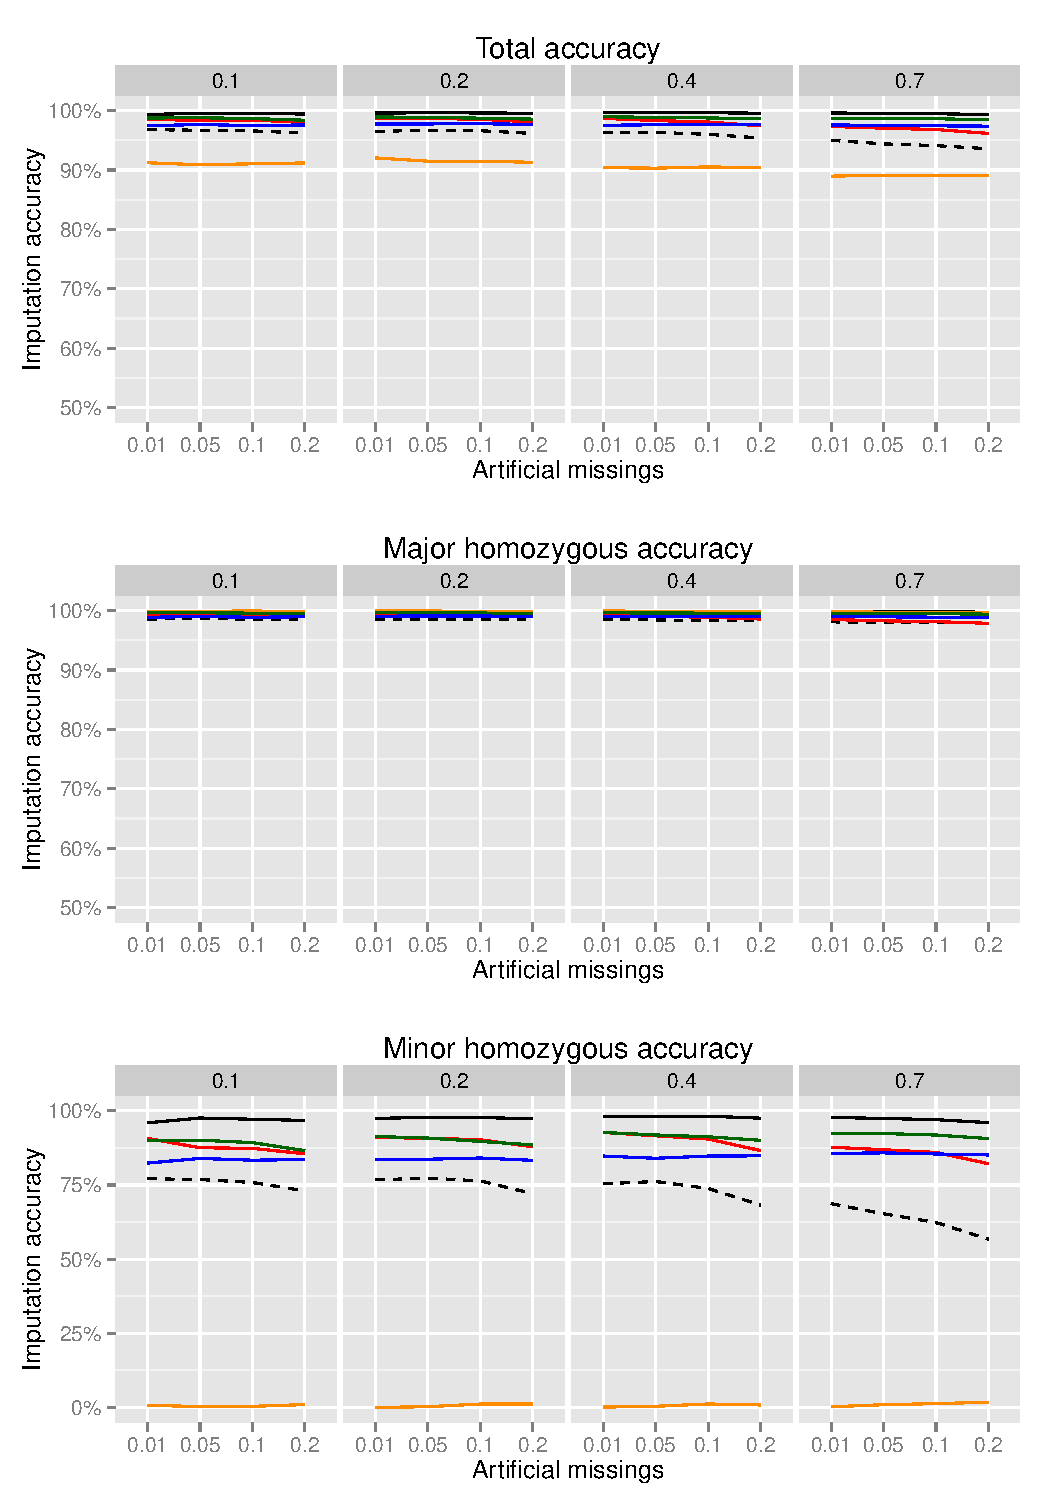
\includegraphics[width=0.95\textwidth]{SupplFig07_Rice-chrom-4.pdf}\caption{
imputation accuracies overall, for the major homozygous genotype (AA) and for the minor homozygous genotype (BB) in datasets consisting of
10\%, 20\%, 40\% and 70\% allowed missing data per locus (boxes) with 1\%, 5\%, 10\% and 20\%
additional missing values artificially introduced (x-axis) for rice chromosome 4 data.
Lines colors represent the five imputation algorithms: MNI
(orange), KNNI (red), SVDI (blue), RFI (green) and Beagle (black)}\end{figure}
\begin{figure}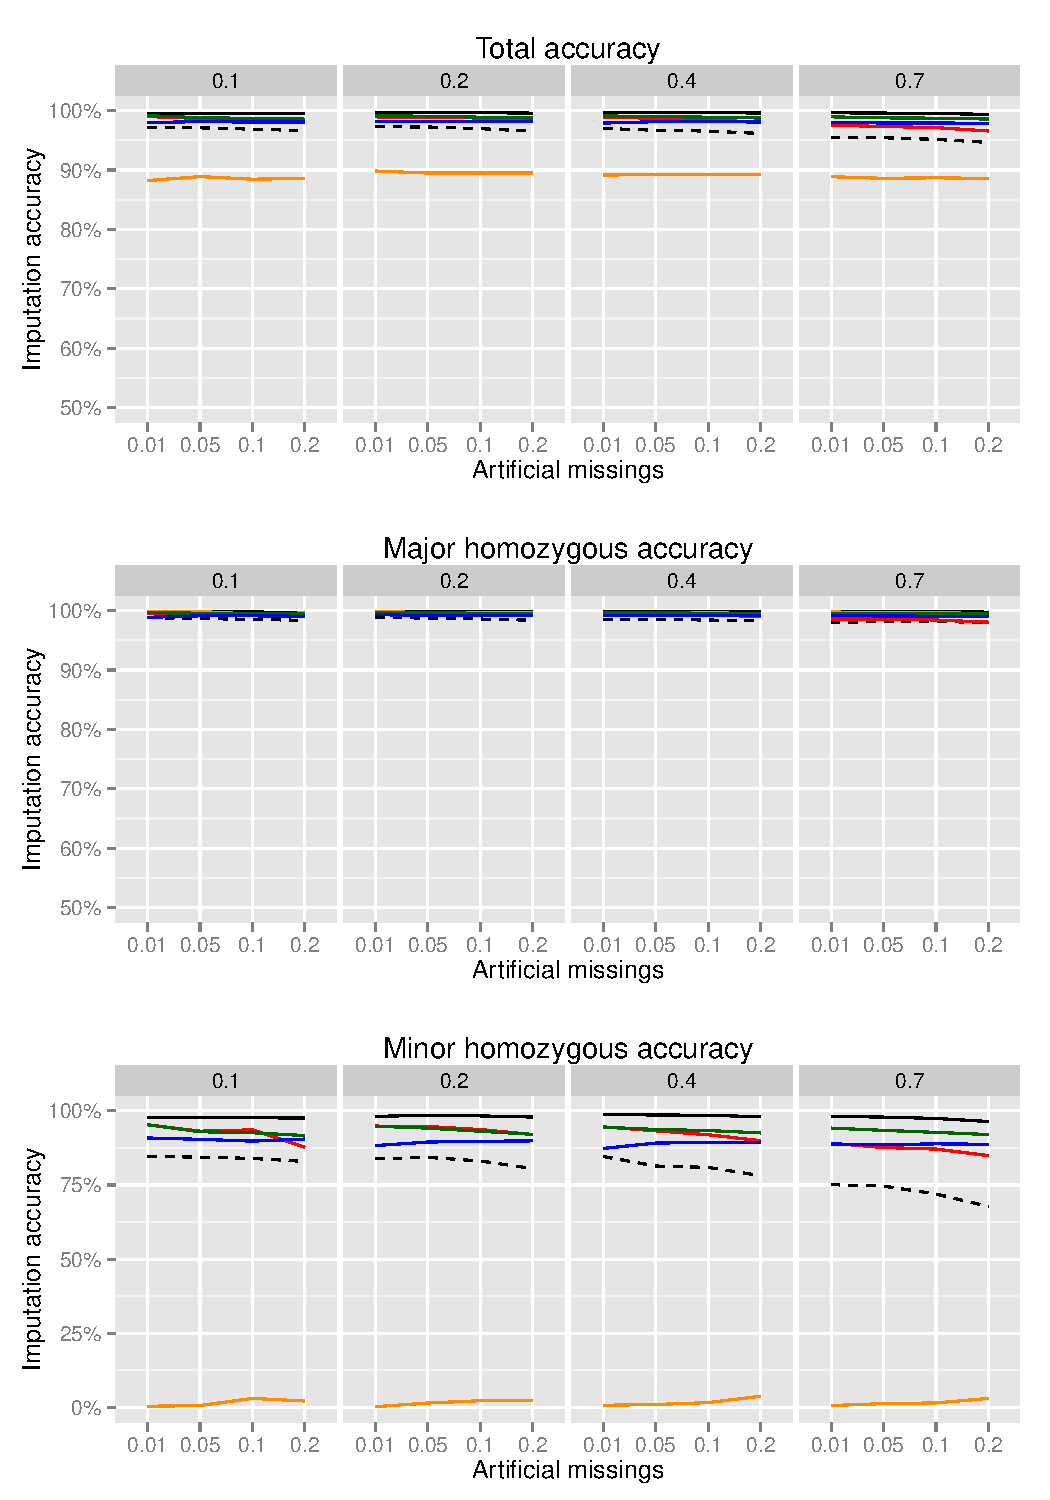
\includegraphics[width=0.95\textwidth]{SupplFig08_Rice-chrom-5.pdf}\caption{
imputation accuracies overall, for the major homozygous genotype (AA) and for the minor homozygous genotype (BB) in datasets consisting of
10\%, 20\%, 40\% and 70\% allowed missing data per locus (boxes) with 1\%, 5\%, 10\% and 20\%
additional missing values artificially introduced (x-axis) for rice chromosome 5 data.
Lines colors represent the five imputation algorithms: MNI
(orange), KNNI (red), SVDI (blue), RFI (green) and Beagle (black)}\end{figure}
\begin{figure}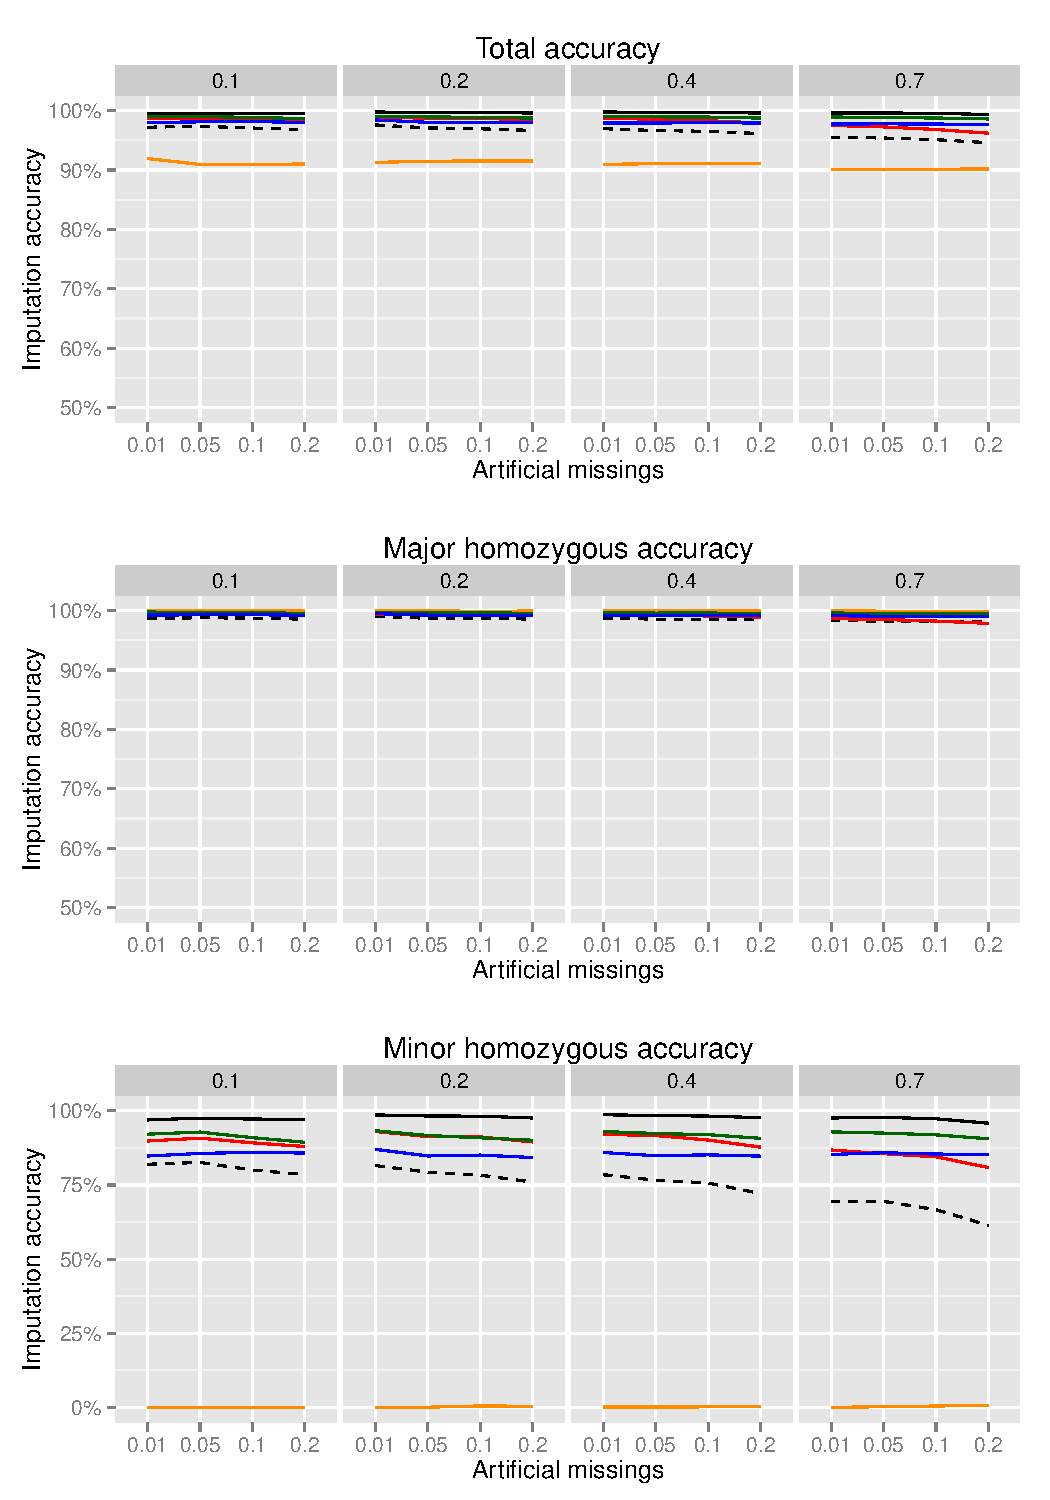
\includegraphics[width=0.95\textwidth]{SupplFig09_Rice-chrom-6.pdf}\caption{
imputation accuracies overall, for the major homozygous genotype (AA) and for the minor homozygous genotype (BB) in datasets consisting of
10\%, 20\%, 40\% and 70\% allowed missing data per locus (boxes) with 1\%, 5\%, 10\% and 20\%
additional missing values artificially introduced (x-axis) for rice chromosome 6 data.
Lines colors represent the five imputation algorithms: MNI
(orange), KNNI (red), SVDI (blue), RFI (green) and Beagle (black)}\end{figure}
\begin{figure}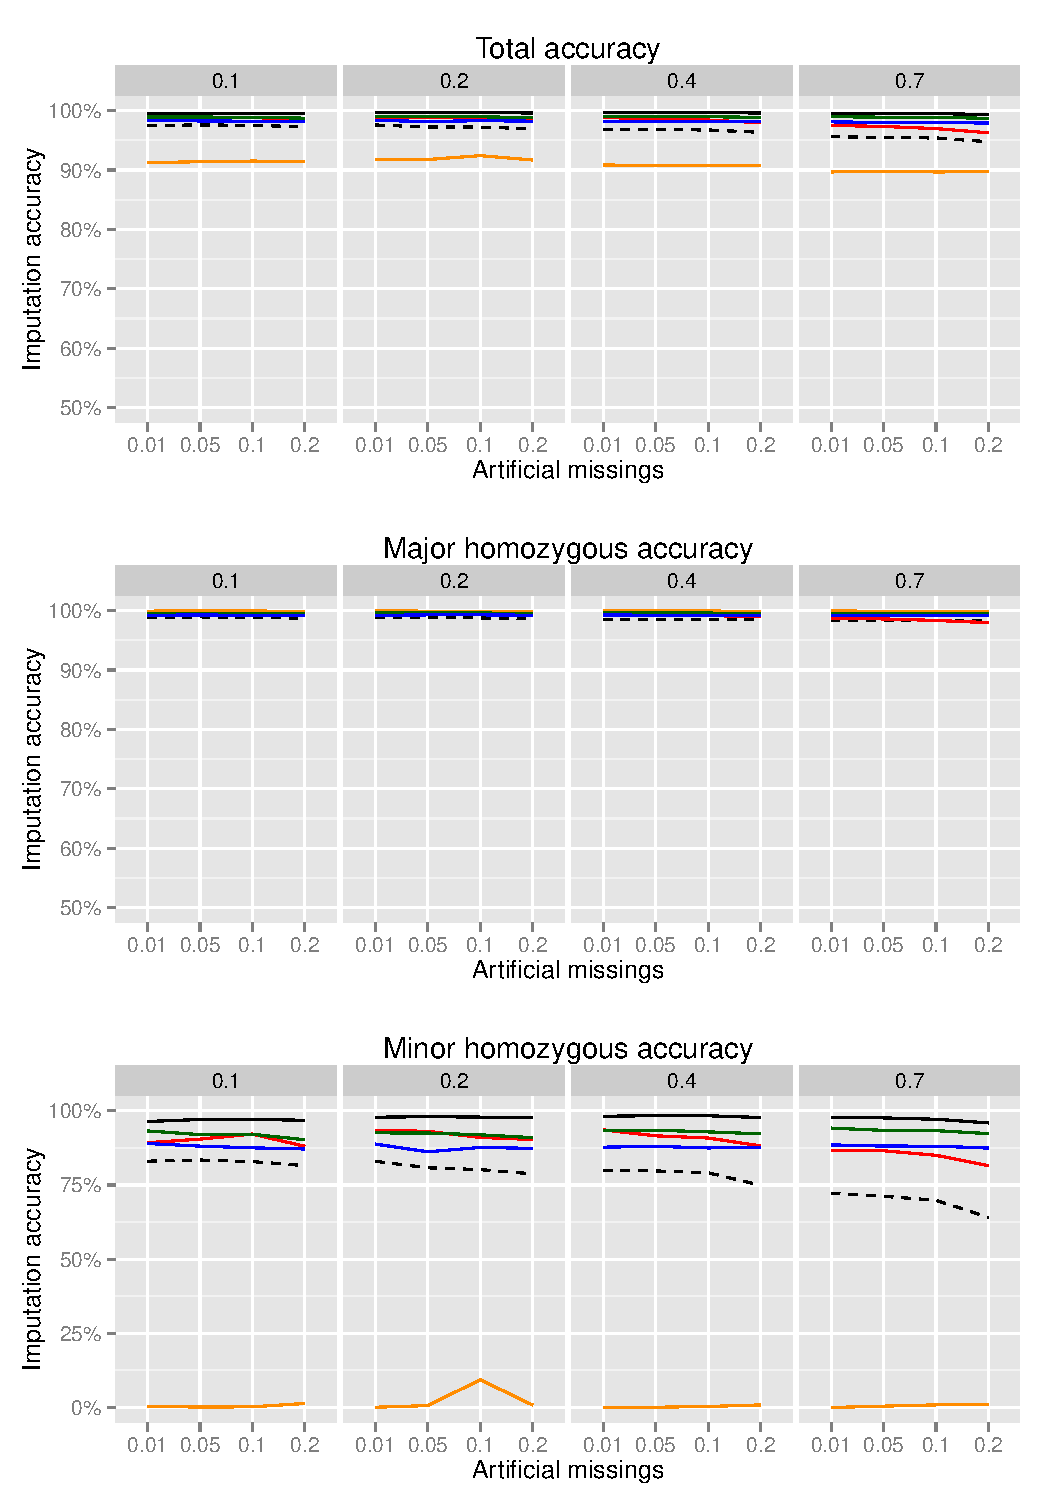
\includegraphics[width=0.95\textwidth]{SupplFig10_Rice-chrom-7.pdf}\caption{
imputation accuracies overall, for the major homozygous genotype (AA) and for the minor homozygous genotype (BB) in datasets consisting of
10\%, 20\%, 40\% and 70\% allowed missing data per locus (boxes) with 1\%, 5\%, 10\% and 20\%
additional missing values artificially introduced (x-axis) for rice chromosome 7 data.
Lines colors represent the five imputation algorithms: MNI
(orange), KNNI (red), SVDI (blue), RFI (green) and Beagle (black)}\end{figure}
\begin{figure}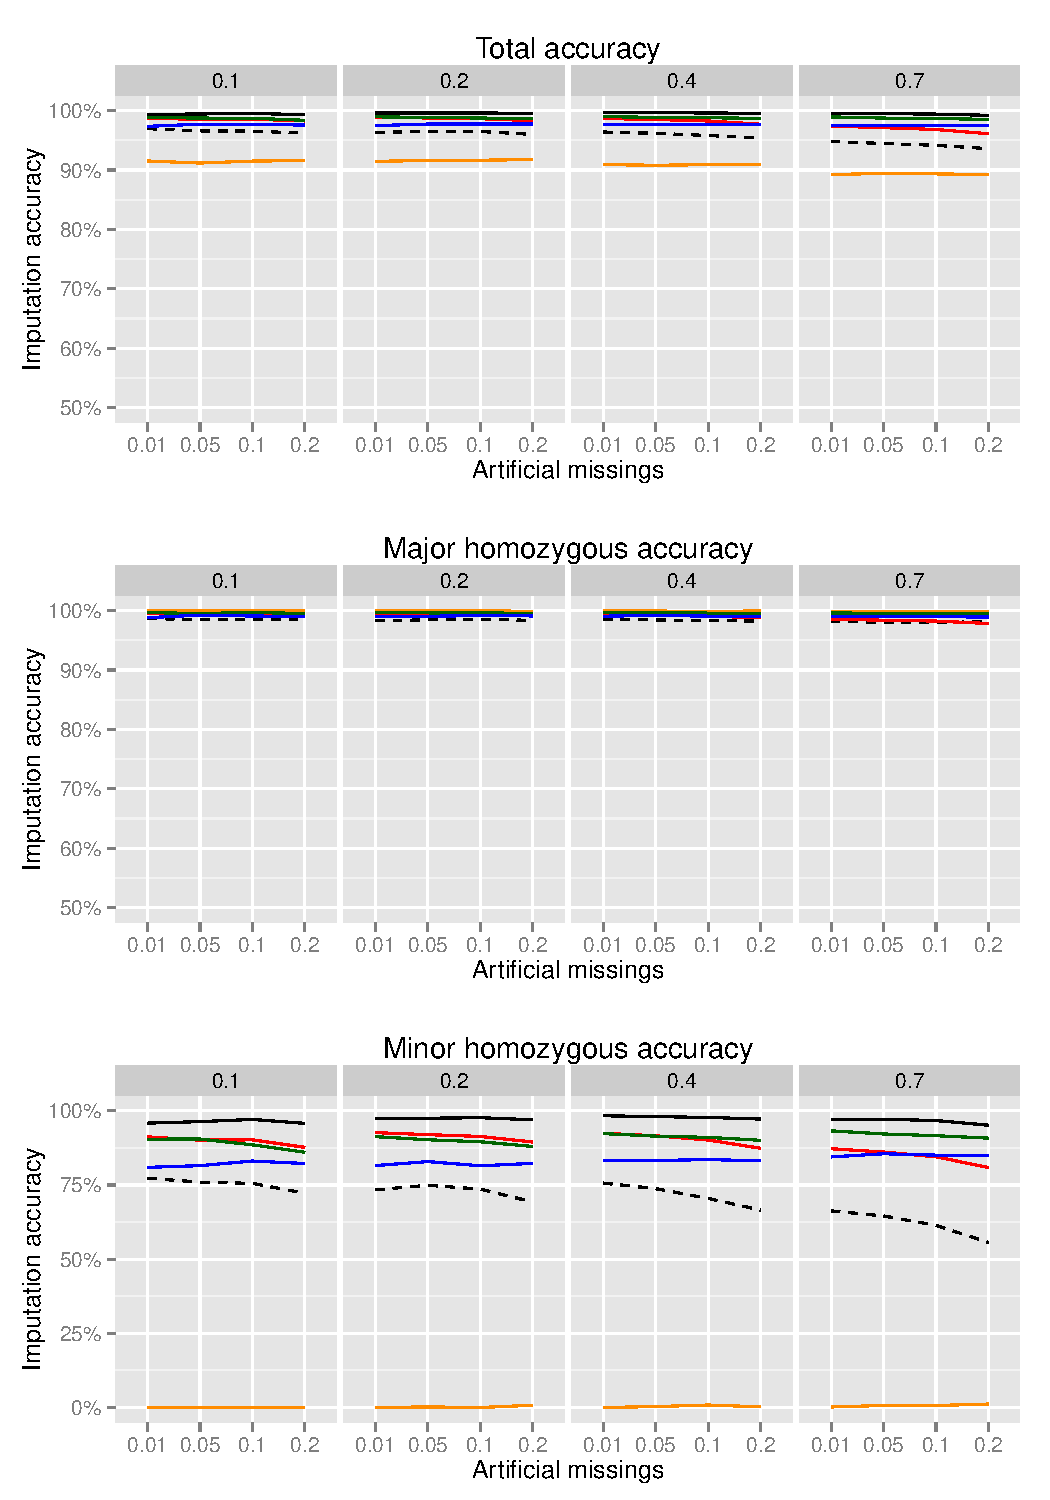
\includegraphics[width=0.95\textwidth]{SupplFig11_Rice-chrom-8.pdf}\caption{
imputation accuracies overall, for the major homozygous genotype (AA) and for the minor homozygous genotype (BB) in datasets consisting of
10\%, 20\%, 40\% and 70\% allowed missing data per locus (boxes) with 1\%, 5\%, 10\% and 20\%
additional missing values artificially introduced (x-axis) for rice chromosome 8 data.
Lines colors represent the five imputation algorithms: MNI
(orange), KNNI (red), SVDI (blue), RFI (green) and Beagle (black)}\end{figure}
\begin{figure}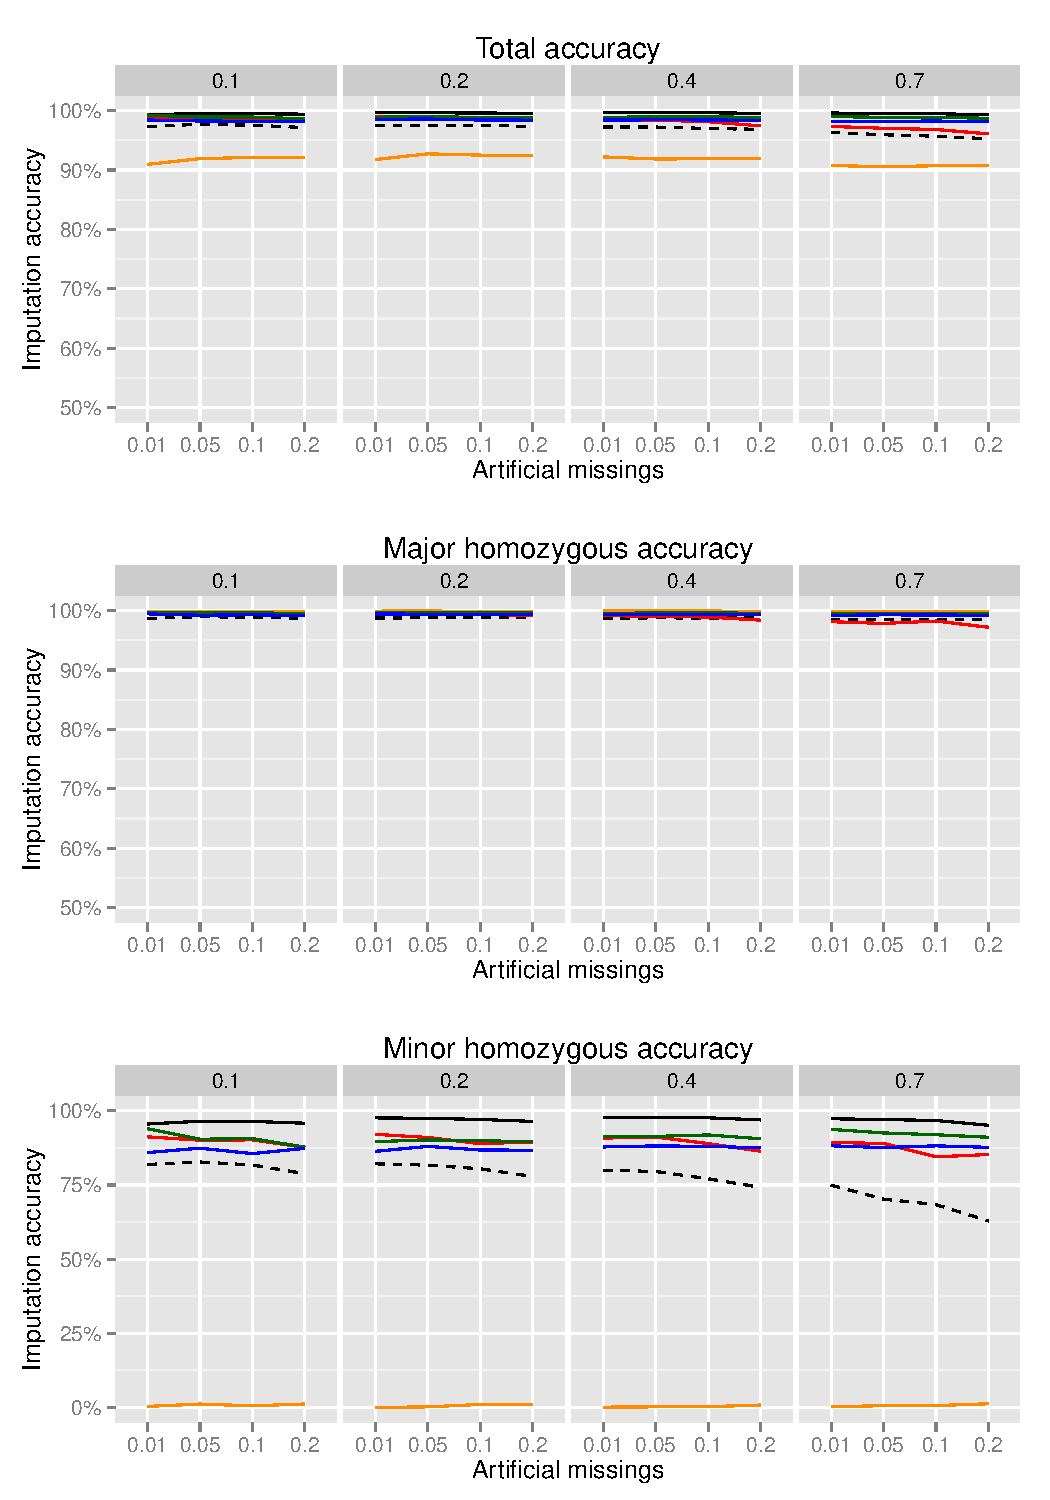
\includegraphics[width=0.95\textwidth]{SupplFig12_Rice-chrom-9.pdf}\caption{
imputation accuracies overall, for the major homozygous genotype (AA) and for the minor homozygous genotype (BB) in datasets consisting of
10\%, 20\%, 40\% and 70\% allowed missing data per locus (boxes) with 1\%, 5\%, 10\% and 20\%
additional missing values artificially introduced (x-axis) for rice chromosome 9 data.
Lines colors represent the five imputation algorithms: MNI
(orange), KNNI (red), SVDI (blue), RFI (green) and Beagle (black)}\end{figure}
\begin{figure}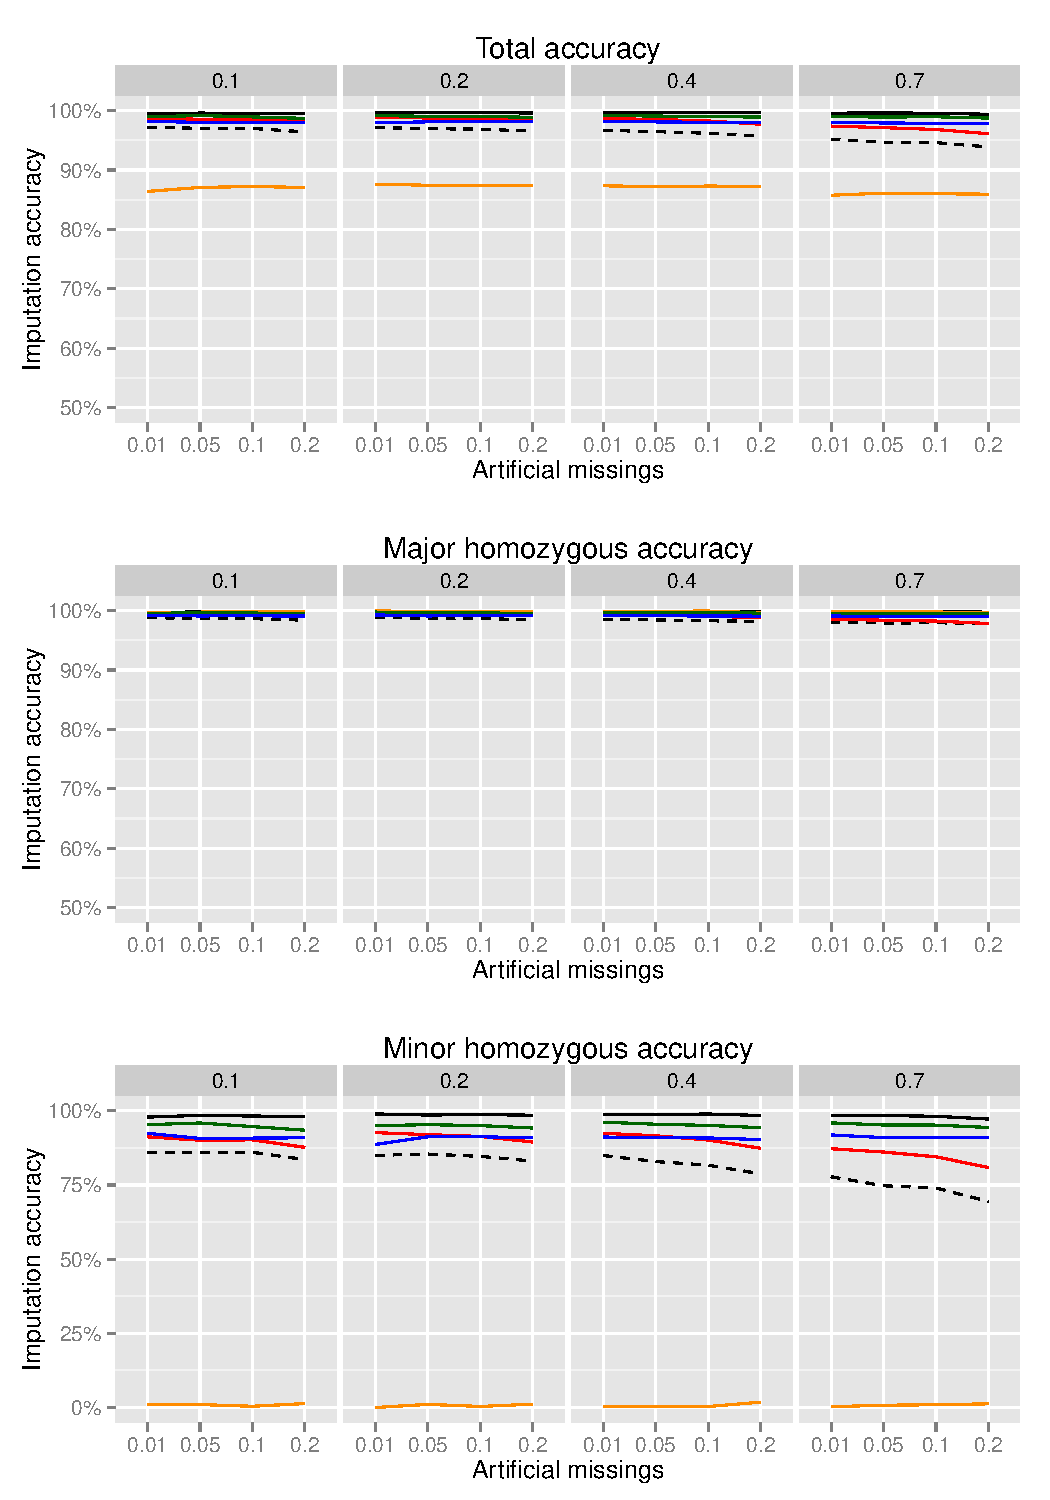
\includegraphics[width=0.95\textwidth]{SupplFig13_Rice-chrom-10.pdf}\caption{
imputation accuracies overall, for the major homozygous genotype (AA) and for the minor homozygous genotype (BB) in datasets consisting of
10\%, 20\%, 40\% and 70\% allowed missing data per locus (boxes) with 1\%, 5\%, 10\% and 20\%
additional missing values artificially introduced (x-axis) for rice chromosome 10 data.
Lines colors represent the five imputation algorithms: MNI
(orange), KNNI (red), SVDI (blue), RFI (green) and Beagle (black)}\end{figure}
\begin{figure}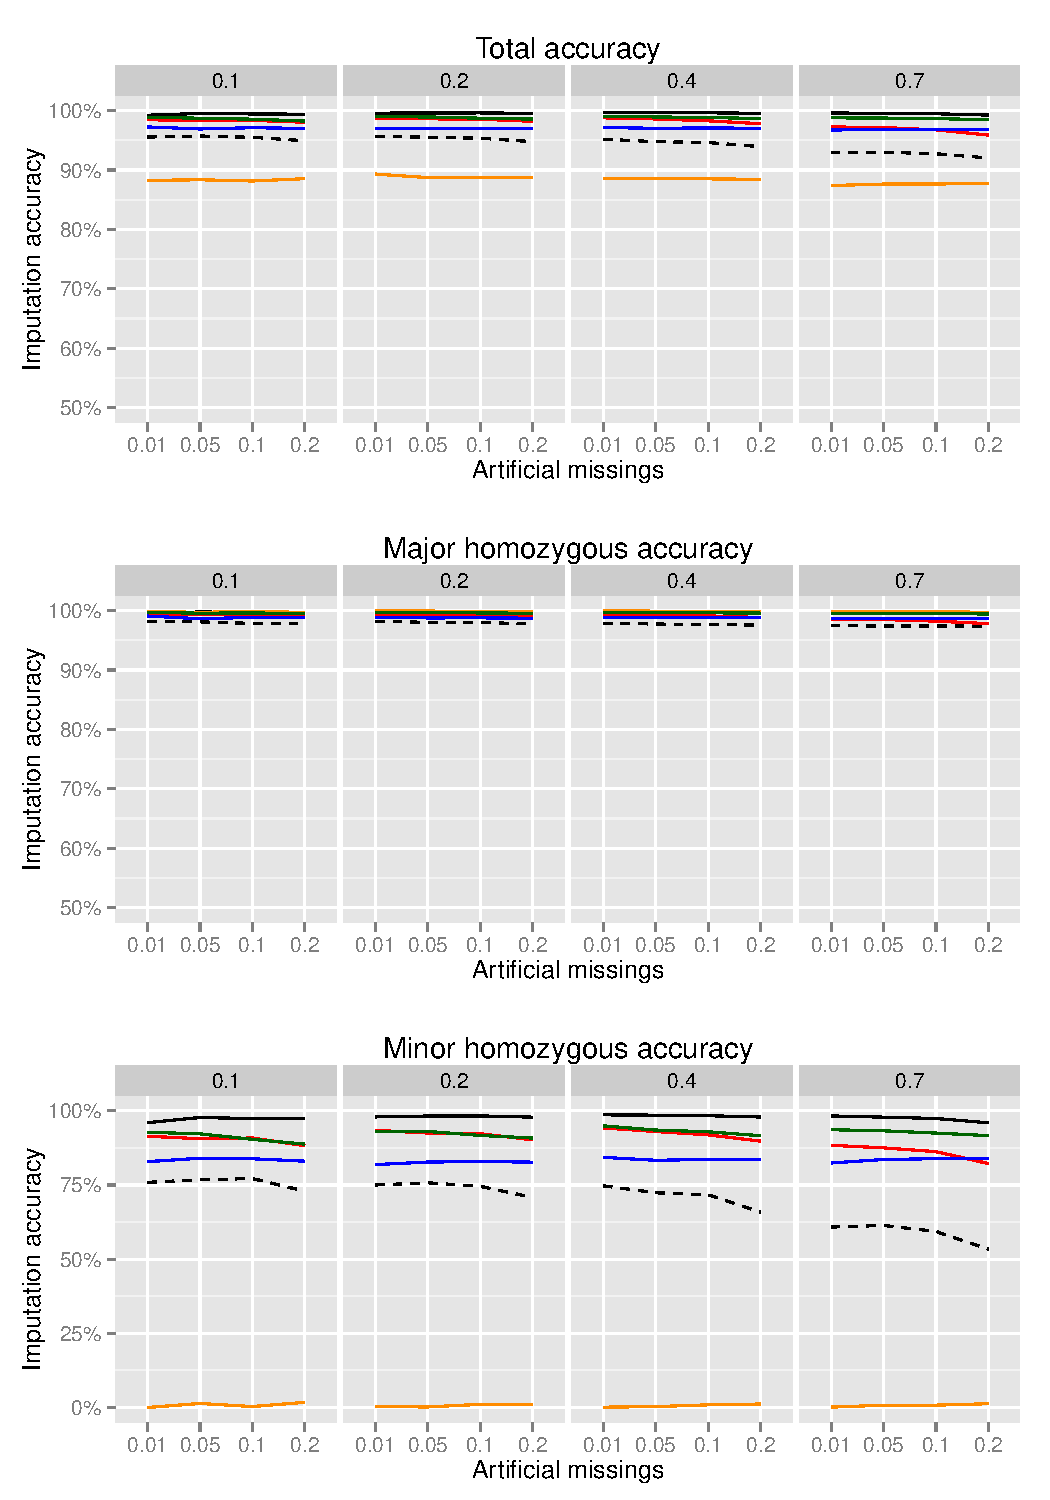
\includegraphics[width=0.95\textwidth]{SupplFig14_Rice-chrom-11.pdf}\caption{
imputation accuracies overall, for the major homozygous genotype (AA) and for the minor homozygous genotype (BB) in datasets consisting of
10\%, 20\%, 40\% and 70\% allowed missing data per locus (boxes) with 1\%, 5\%, 10\% and 20\%
additional missing values artificially introduced (x-axis) for rice chromosome 11 data.
Lines colors represent the five imputation algorithms: MNI
(orange), KNNI (red), SVDI (blue), RFI (green) and Beagle (black)}\end{figure}
\begin{figure}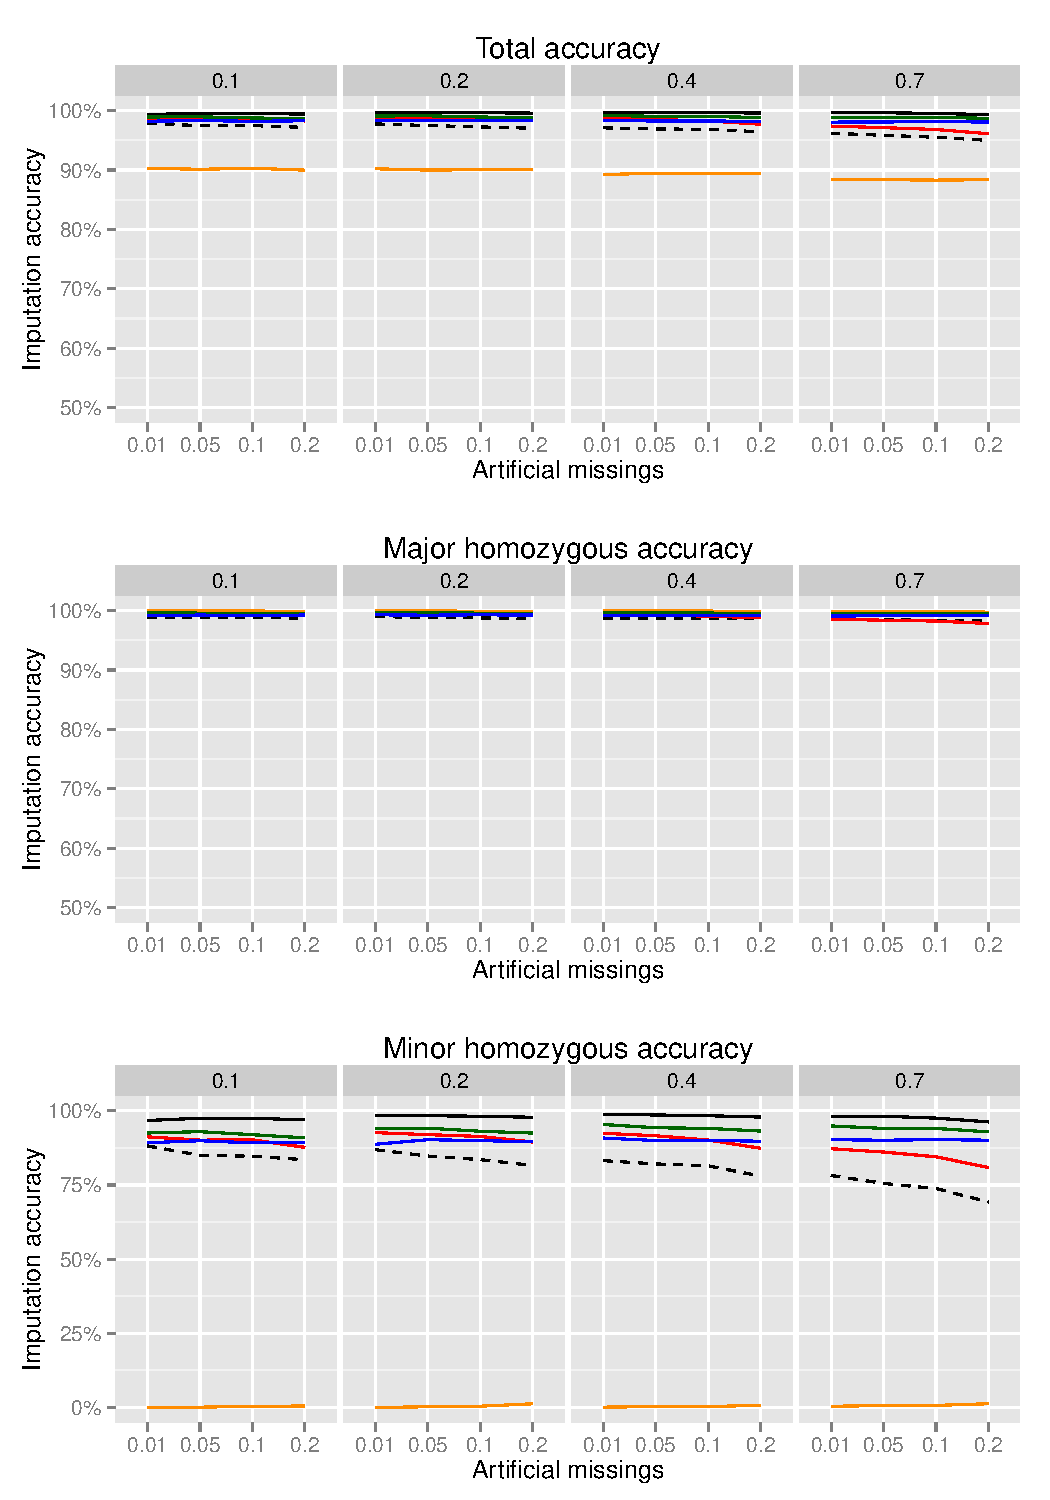
\includegraphics[width=0.95\textwidth]{SupplFig15_Rice-chrom-12.pdf}\caption{
imputation accuracies overall, for the major homozygous genotype (AA) and for the minor homozygous genotype (BB) in datasets consisting of
10\%, 20\%, 40\% and 70\% allowed missing data per locus (boxes) with 1\%, 5\%, 10\% and 20\%
additional missing values artificially introduced (x-axis) for rice chromosome 12 data.
Lines colors represent the five imputation algorithms: MNI
(orange), KNNI (red), SVDI (blue), RFI (green) and Beagle (black)}\end{figure}
\begin{figure}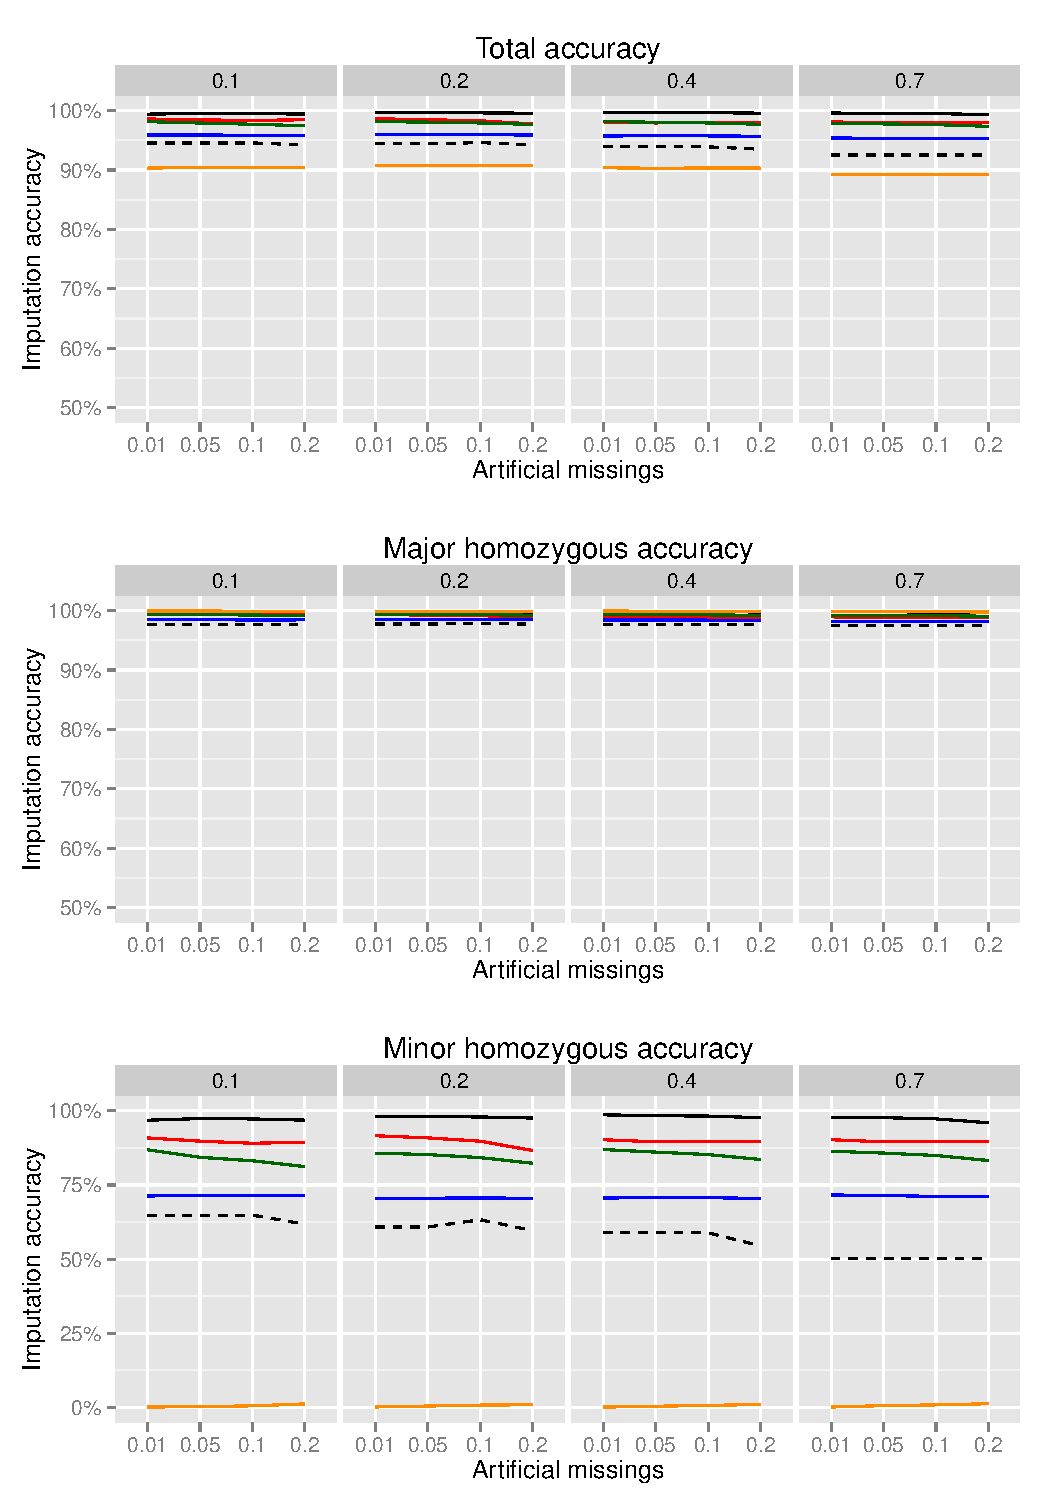
\includegraphics[width=0.95\textwidth]{SupplFig16_Rice.pdf}\caption{
imputation accuracies overall, for the major homozygous genotype (AA) and for the minor homozygous genotype (BB) in datasets consisting of
10\%, 20\%, 40\% and 70\% allowed missing data per locus (boxes) with 1\%, 5\%, 10\% and 20\%
additional missing values artificially introduced (x-axis) for whole rice data set.
Lines colors represent the five imputation algorithms: MNI
(orange), KNNI (red), SVDI (blue), RFI (green) and Beagle (black)}\end{figure}

\subsection{SNP calling thresholds}
\label{sec:SNP_calling_thresholds}
Genotype calling can incur in two types of error, namely when a heterozygote is wrongly identified as homozigote (HET->HOM) and the reverse case (HOM->HET). 

Without considering sequencing errors due to the machine1




